\subsubsection{summary-suGlobalManagementOfEvent}

\label{RE-use-case-suGlobalManagementOfEvent}


Shows the suGlobaManagementOfEvent use-case and its actors.		  


\begin{usecase}
  \addheading{Use-Case Description}
  \addsingletwocolumnrow{Name}{suGlobalManagementOfEvent}
  \addsingletwocolumnrow{Scope}{system}
  \addsingletwocolumnrow{Level}{summary}
  

\addrowheading{Primary actor(s)}
\addnumberedsinglerow{}{\msrcode{actCentralCoordinator[active]}}


\addrowheading{Secondary actor(s)}
\addnumberedsinglerow{}{\msrcode{actCommunicationCompany[active]}}
\addnumberedsinglerow{}{\msrcode{actFiremenCoordinator[active]}}
\addnumberedsinglerow{}{\msrcode{actPoliceCoordinator[active]}}
\addnumberedsinglerow{}{\msrcode{actTowServiceCoordinator[active]}}

\addrowheading{Goal(s) description}
\addsinglerow{Shows the suGlobaManagementOfEvent use-case and its actors.}

\addrowheading{Reuse}
\addnumberedsinglerow{}{\msrucname{oeRequestCrisisEventLocation [0..*]}}
\addnumberedsinglerow{}{\msrucname{oeReceiveCrisisEventLocation [0..*]}}
\addnumberedsinglerow{}{\msrucname{oeConfirmCrisisEventLocation [1..*]}}
\addnumberedsinglerow{}{\msrucname{oeCreateNewCrisisEvent [1..*]}}
\addnumberedsinglerow{}{\msrucname{oeUpdateDispatchStatus [4..*]}}
\addnumberedsinglerow{}{\msrucname{oeRequestHelp [0..*]}}

\addrowheading{Protocol condition(s)}
\addnumberedsinglerow{}{
}

\addrowheading{Pre-condition(s)}
\addnumberedsinglerow{}{
}

\addrowheading{Main post-condition(s)}
\addnumberedsinglerow{}{
}

\addrowheading{Main Steps}
\addalphanumberedsinglerow{}{the actor \msrcode{actCentralCoordinator} executes the \msrucname{oeRequestCrisisEventLocation} use case}
\addalphanumberedsinglerow{}{the actor \msrcode{actCommunicationCompany} executes the \msrucname{oeReceiveCrisisEventLocation} use case}
\addalphanumberedsinglerow{}{the actor \msrcode{actCentralCoordinator} executes the \msrucname{oeConfirmCrisisEventLocation} use case}
\addalphanumberedsinglerow{}{the actor \msrcode{actCentralCoordinator} executes the \msrucname{oeCreateNewCrisisEvent} use case}
\addalphanumberedsinglerow{}{the actor \msrcode{actFiremenCoordinator} executes the \msrucname{oeUpdateDispatchStatus} use case}
\addalphanumberedsinglerow{}{the actor \msrcode{actTowServiceCoordinator} executes the \msrucname{oeRefreshMap} use case}
\addalphanumberedsinglerow{}{the actor \msrcode{actTowServiceCoordinator} executes the \msrucname{oeMessage} use case}
\addalphanumberedsinglerow{}{the actor \msrcode{actTowServiceCoordinator} executes the \msrucname{oeUpdateDispatchStatus} use case}
\addalphanumberedsinglerow{}{the actor \msrcode{actFiremenCoordinator} executes the \msrucname{oeRequestHelp} use case}
\addalphanumberedsinglerow{}{the actor \msrcode{actPoliceCoordinator} executes the \msrucname{oeUpdateDispatchStatus} use case}
\addrowheading{Steps Ordering Constraints}
\addnumberedsinglerow{}{if (b) then previously (a)}
\addnumberedsinglerow{}{step (c) must be executed before step (d)}
\addnumberedsinglerow{}{step (d) must be executed before the step (e) to (j)}
\addnumberedsinglerow{}{step (e) must be executed at least two times}
\addnumberedsinglerow{}{step (h) must be executed at least two times}
\addnumberedsinglerow{}{step (j) can only be executed if step (i) has at least been executed once previously}
\addnumberedsinglerow{}{step (j) must be executed at least two times}

\addrowheading{Additional Information}
\addsinglerow{
none
}

\end{usecase} 


Figure \ref{fig:lu.uni.lassy.excalibur.group09.spec-RE-UCD-uc-suGlobalManagementOfEvent}
Shows the suGlobaManagementOfEvent use-case and its actors.

\begin{figure}[htbp]
\begin{center}

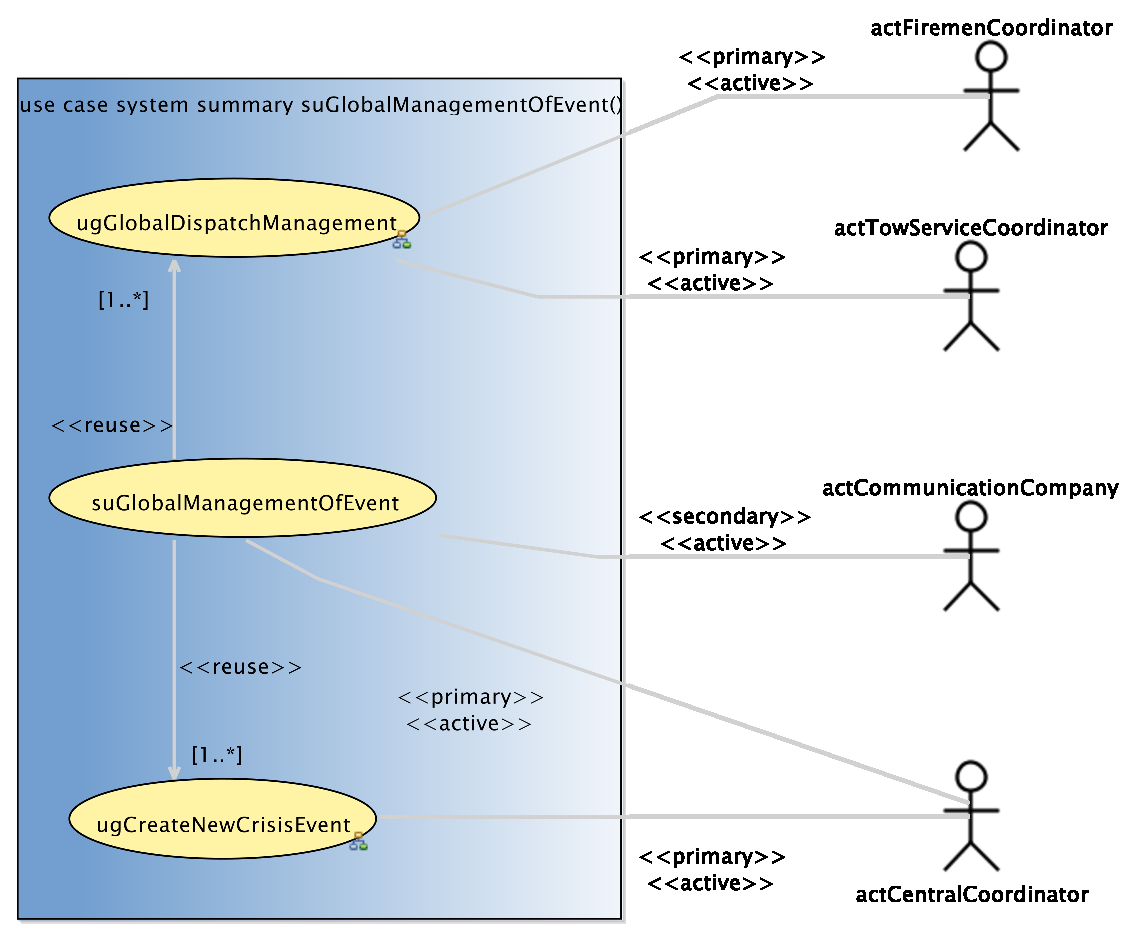
\includegraphics[
angle=0
,width=1.0\textwidth
]{./images-report-gen/usecase-model/summary/uc-suGlobalManagementOfEvent.eps}
\end{center}
\caption[lu.uni.lassy.excalibur.group09.spec Use Case Diagram: uc-suGlobalManagementOfEvent]{}
\label{fig:lu.uni.lassy.excalibur.group09.spec-RE-UCD-uc-suGlobalManagementOfEvent}
\end{figure}
\vspace{0.5cm}
